\documentclass[11pt]{article}
\usepackage{appendix}
\usepackage{amsmath,amssymb,amsthm, enumerate,epsfig}
\usepackage{ifthen,latexsym,syntonly}
\usepackage{fullpages}
\usepackage{epsfig}
\usepackage{comment}
\usepackage{booktabs}
\usepackage{tabularx}
\usepackage{subcaption}
%\usepackage{hyperref}
%\usepackage[normalem]{ulem}
\usepackage[Figure sright]{rotating}
\newcommand{\Lower}[1]{\smash{\lower 1.5ex \hbox{#1}}}
\newcommand{\STRUT}{\rule{0in}{3ex}}
\newcommand{\BSTRUT}{\rule[-1.2ex]{0pt}{0pt}}


%\usepackage[showrefs]{refcheck}  %use this to show equation and section labels
\usepackage{color,colortbl}
\definecolor{LightCyan}{rgb}{0.88,1,1}
\usepackage[round,comma,authoryear]{natbib}   % for natbib
%\usepackage{subfigure}
%\usepackage{caption,subcaption}
\bibliographystyle{mynat}   % for natbib
%\bibpunct{(}{)},{a}{},  % for natbib
%                            % need to have mynat.bst in an accessible directory


\bibpunct{(}{)},{a}{},  % for natbib
                            % need to have mynat.bst in an accessible directory
\usepackage{setspace}
\onehalfspacing

\newtheorem{theorem}{Theorem}[section]
\newtheorem{remark}[theorem]{Remark}
\newtheorem{assumption}[theorem]{Assumption}
%\newtheorem{case}[theorem]{Case}
\newtheorem{claim}[theorem]{Claim}
%\newtheorem{conclusion}[theorem]{Conclusion}
\newtheorem{corollary}[theorem]{Corollary}
\newtheorem{condition}[theorem]{Condition}
\newtheorem{criterion}[theorem]{Criterion}
\newtheorem{definition}[theorem]{Definition}
\newtheorem{example}[theorem]{Example}
\newtheorem{lemma}[theorem]{Lemma}
\newtheorem{problem}[theorem]{Problem}
\newtheorem{proposition}[theorem]{Proposition}
%\newtheorem{solution}[theorem]{Solution}
%\newtheorem{summary}[theorem]{Summary}
\newtheorem{thm}[theorem]{Theorem}

\newcommand{\TS}[1]{{\textcolor{red}{#1}}}
\newcommand{\GH}[1]{{\textcolor{blue}{#1}}}

%%%%%%%%%%%%%%%%%%%%%%%%%%%%%%%%%%%%%%%%%%%%%%%%%%%%%%%%%%%%%%%%%%%%%%%%%%%
%
%

\title{Pennsylvania State Finances: 1820 to 1860\footnote{ 
We thank William Berkley for supporting our research. 
Hall thanks the Theodore and Jane Norman Fund for financial support.}}

\author{GJH\footnote{Brandeis University, E-mail: ghall@brandeis.edu.} \and
TJS\footnote{New York University, E-mail: thomas.sargent@nyu.edu.}}


\begin{document}
\graphicspath{{Penn_figures/}}

\maketitle

%\begin{abstract}
%\noindent 
%abstract here
%\end{abstract}

%\noindent \textbf{Keywords}:


\section{Summary}


This document reports tables and figures that might find their way into 
a chapter on early state finance.  New York might be the ``good" case study.  Pennsylvania might
be the ``bad" case study.


\section{The Government Budget Constraints}

The organizing principle is the government budget constraint with private assets (which we labeled ``state funds" in the New York memo and call ``state assets" in this memo).  
\begin{eqnarray}
\underbrace{G_t}_{\substack{\text{government}\\\text{spending}}}  + \underbrace{r_t^B B_{t-1}}_{\substack{\text{interest on}\\\text{state debt}}} + \underbrace{A_t - A_{t-1}}_{\substack{\text{change in}\\ \text{state funds}}} \; = \; \; \underbrace{T_t}_{\text{taxes}}
\; \; + \; \; \underbrace{r_t^A A_{t-1}}_{\substack{\text{interest on}\\ \text{state funds}}}  \; \;  +  \; \; \underbrace{B_t - B_{t-1}}_{\substack{\text{change in}\\ \text{state debt}}} 
\label{eq:penn_consolidated_bc}
\end{eqnarray}



\section{Pennsylvania Revenues and Expenditures}

In figure~\ref{fig:penn_rev_exp}, I plot total revenues and expenditures (including interest payments 
and defaulted payments).  In figure~\ref{fig:penn_deficits}, I plot gross and primary deficits

\begin{itemize}

\item Unlike New York, Pennsylvania included public works spending and revenues directly in its general account.

\item The 1836-1837 spike in revenue is due to the federal government's payment of surplus federal funds to the states and unusually large fees received from bank charters.

\item In figure~\ref{fig:penn_deficits} we see large deficits before the crisis.  After the crisis, the Commonwealth ran 
a primary surplus and a balanced (gross) budget. 

\end{itemize}

\begin{figure}
\center{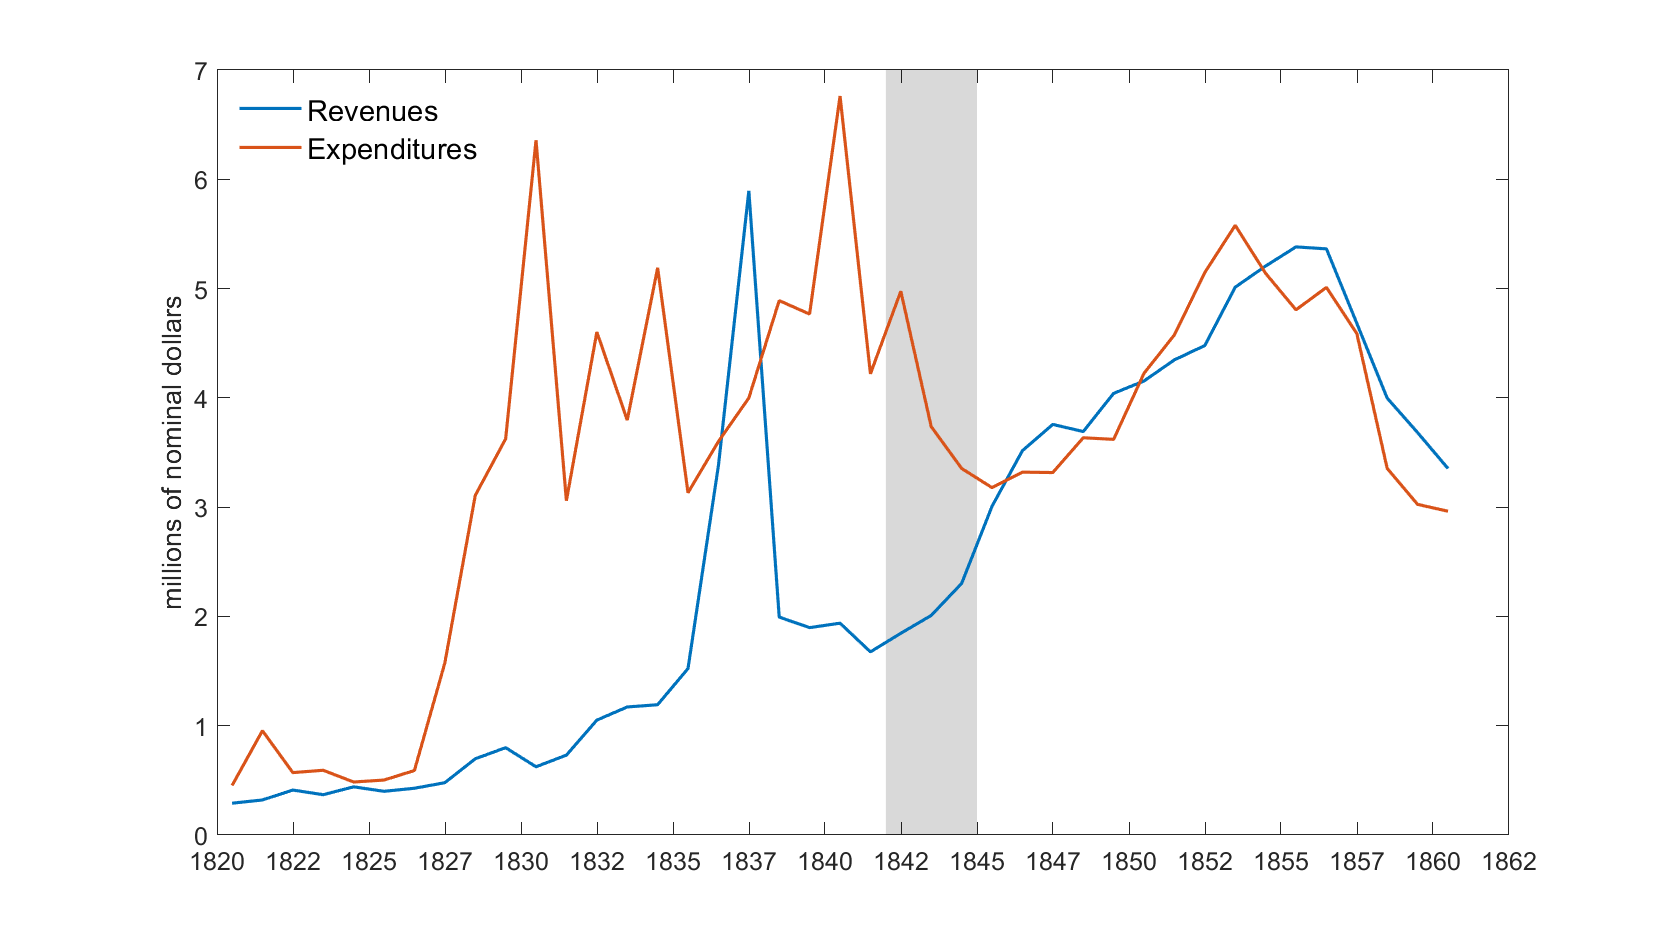
\includegraphics[scale=0.50]{penn_revenue_expend.png}}
\caption{Pennsylvania State Revenue and Expenditures}
\flushleft{\footnotesize The period of default (1842-1844) is shaded in grey.}
\label{fig:penn_rev_exp}

\center{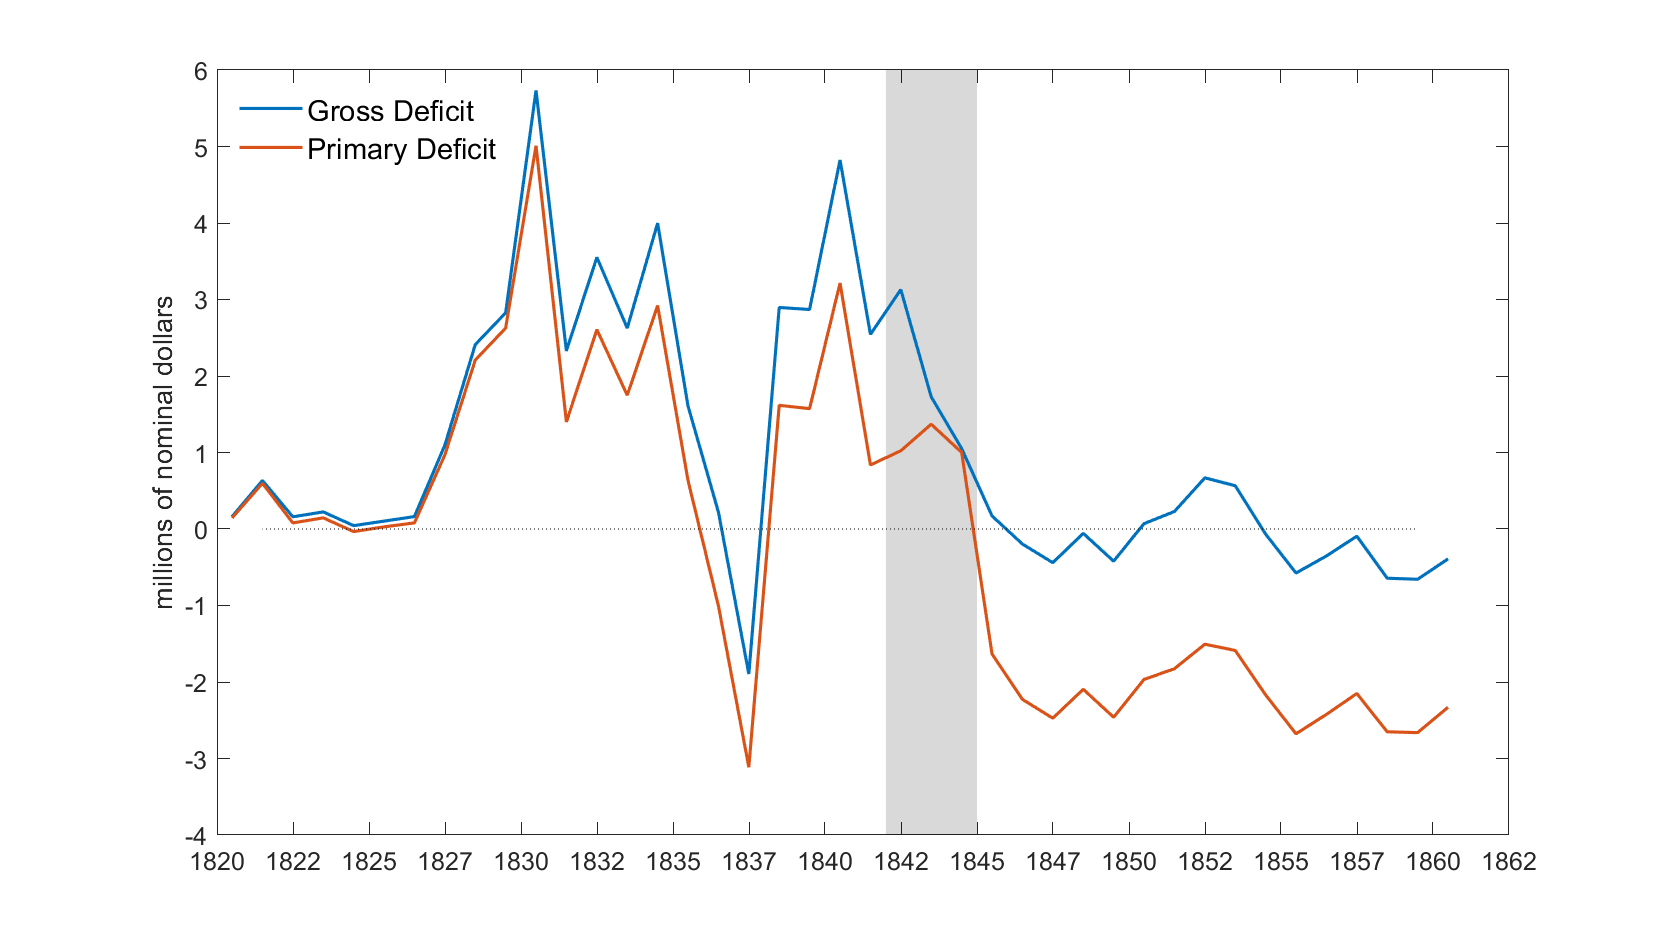
\includegraphics[scale=0.50]{penn_deficit.png}}
\caption{Pennsylvania Gross and Primary Deficits}
\flushleft{\footnotesize The period of default (1842-1844) is shaded in grey.}
\label{fig:penn_deficits}
\end{figure}


\noindent In figure~\ref{fig:penn_revenues}, I plot the sources of 
Commonwealth revenues from 1820 to 1860

\begin{itemize}

\item Land sales make up a relatively small share of total revenue.  This 
is similar to New York State.  Unlike New York, revenue from state assets is a 
small share of total revenue.  See figure 12 of the New York State memo.

\item The large revenues from the Other category in 1836 and 1837 are from 
``Enrollment of Bank Charters.''

\item The large payment from the federal government is the distribution of the 
federal surplus to the states mandated by the Deposit Act of 1836.

\item Tax revenue increased starting in 1845, as a large number of new taxes 
were introduced.

\end{itemize}

\begin{figure}
\center{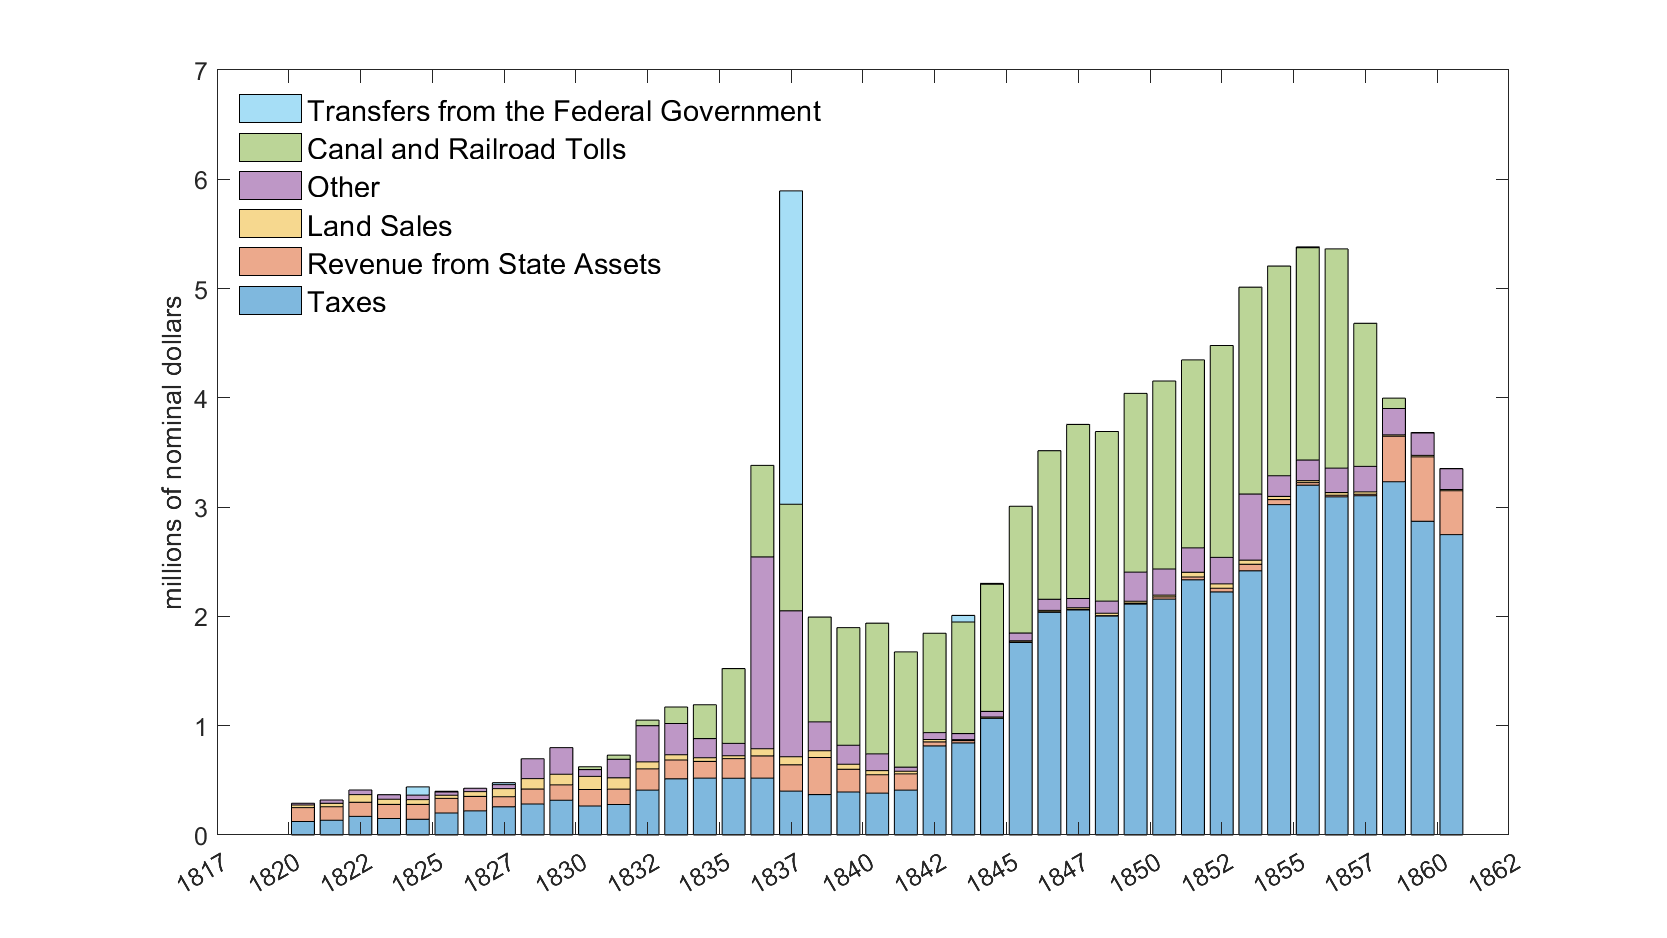
\includegraphics[scale=0.50]{penn_revenues.png}}
\caption{Pennsylvania Revenues}
\label{fig:penn_revenues}


\center{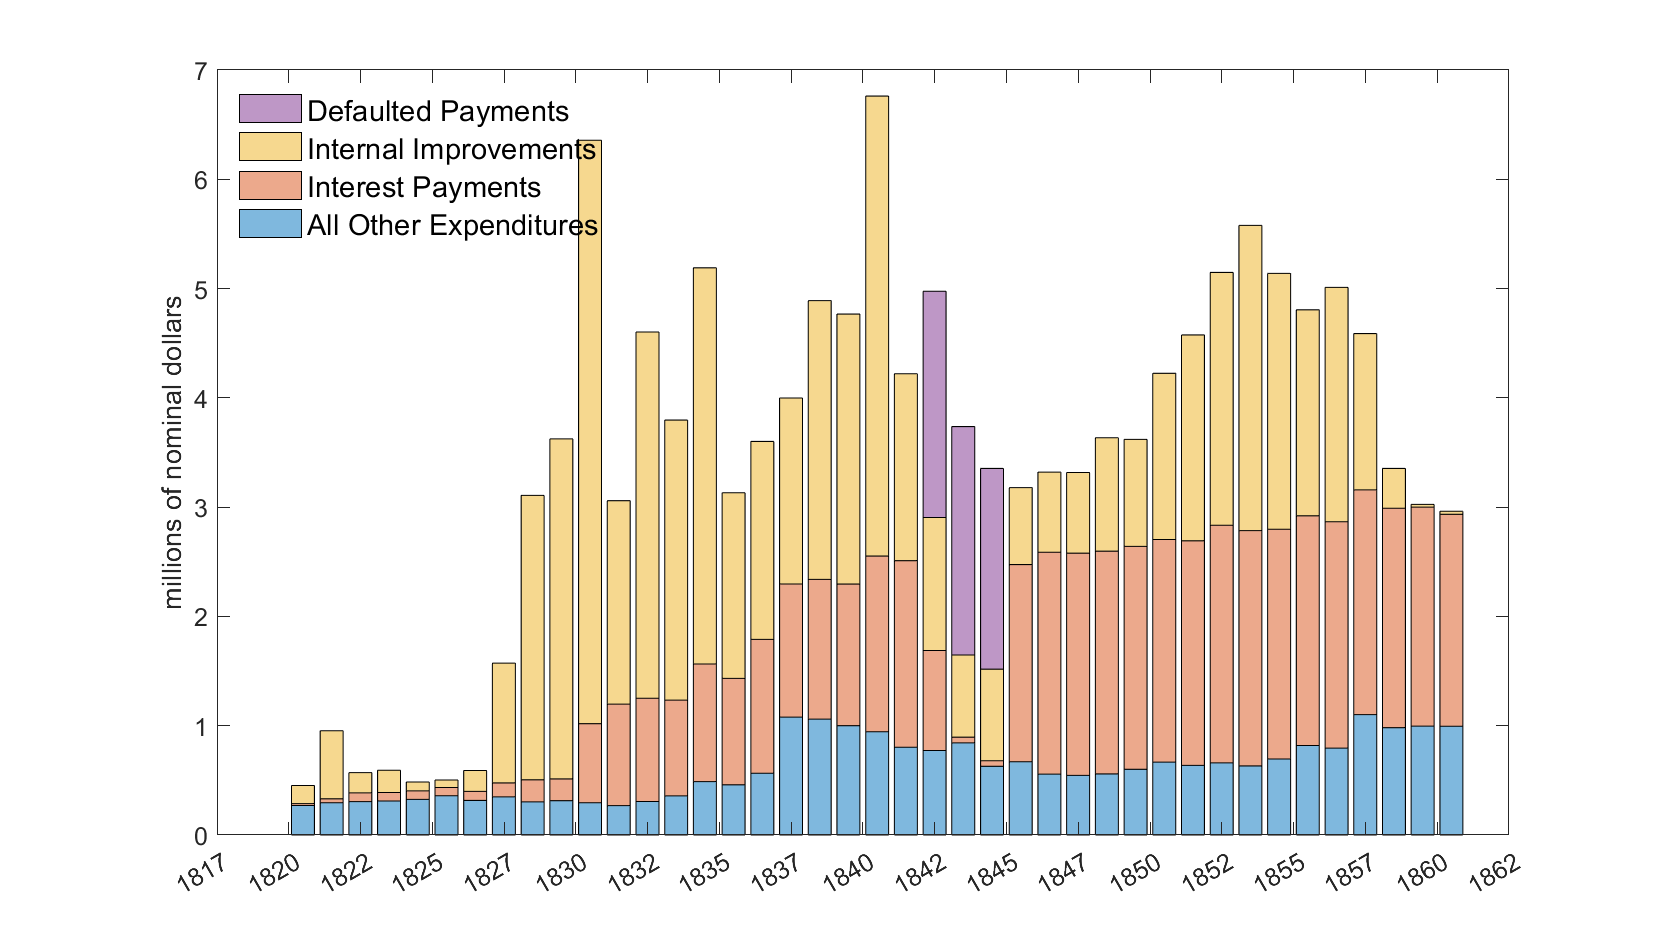
\includegraphics[scale=0.50]{penn_expenditures.png}}
\caption{Pennsylvania Expenditures}
\label{fig:penn_expenditures}
\end{figure}


\noindent In figure~\ref{fig:penn_expenditures}, I plot expenditure components over time.
\begin{itemize}

\item Spending on internal improvements and interest payments is far and 
away the largest spending categories.

\item 1842, 1843, and 1844, Pennsylvania failed to make interest and other 
promised payments.  As discussed below, bondholders were issued ``interest 
certificates," and other non-payments to government contractors were recorded 
as ``domestic creditors."  These defaulted payments are reported in purple.

\item Compare this figure to figures 8 and 11 in the New York State memo. In 
Pennsylvania, interest payments made up a much larger share of expenditures 
than they did in New York.

\end{itemize}

\section{Debt and Assets}

\noindent I plot the quantity of Pennsylvania State debt in figure~\ref{fig:penn_debt}, 
decomposed by loan purpose.  I also split out the extraordinary ``loans'' issued during the
crisis.

\begin{itemize}

\item Between the early 1825 and 1840, nearly all of the outstanding debt had been issued to fund internal
improvements.  Starting in the 1840s nearly all new debt was issued to rollover past debt or
to make coupon payments. These refinancing loans allowed other revenue to be used to 
finance continued spending on internal improvements.


\item In 1840, Pennsylvania's debt stood at \$33.3 million, and the State 
collected \$1.9 million in total revenue. That same year, New York State's 
consolidated debt was \$17.6 million, and it collected \$2.9 million in total 
revenue (across its general and Canal accounts).

\item From 1838 to 1842, the State Auditor General's and Treasurer's records 
of the State's debts included \$2,867,514.78 as a debt to the federal 
government with the expectation that it would have to be repaid.  Interest 
was never paid on this ``debt," and the federal government never demanded its 
return. New York State never included this obligation in its debt records. We 
exclude this debt in figure~\ref{fig:penn_debt}.

\end{itemize}

\begin{figure}
\center{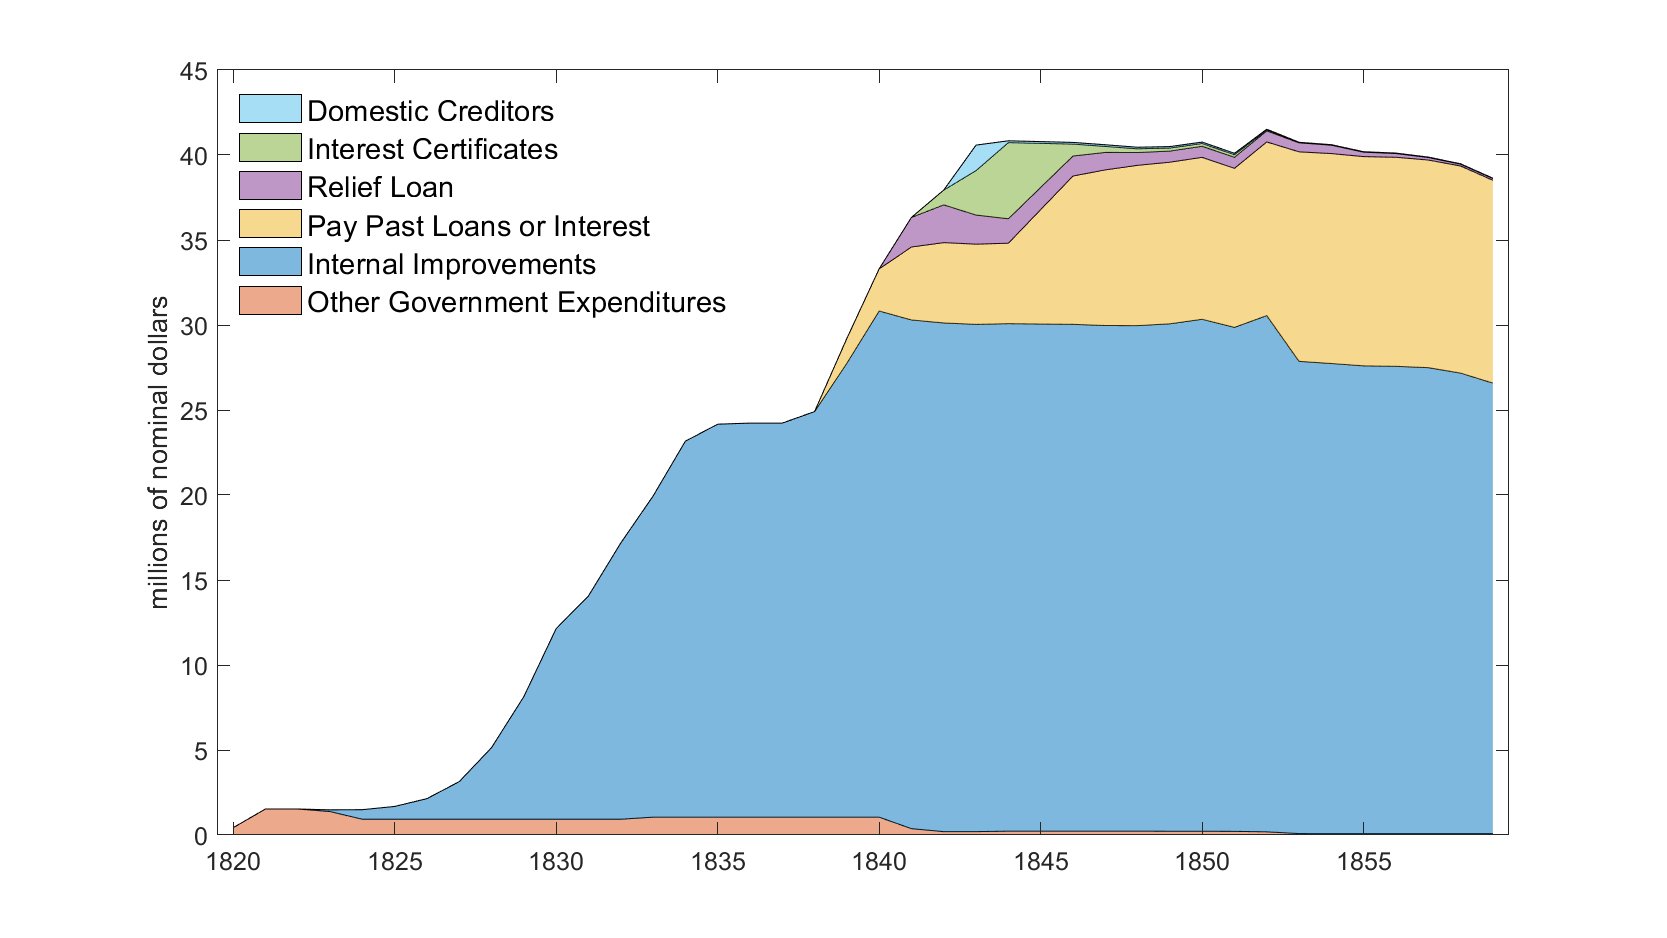
\includegraphics[scale=0.50]{penn_debt_by_purpose.png}}
\caption{Pennsylvania Debt Decomposed by Purpose}
\label{fig:penn_debt}
\end{figure}

\begin{itemize}

\item Pennsylvania owned bank stocks, turnpike and bridge stocks, and canal and 
navigation stocks. I plot the aggregate value of these stocks (reported at 
their par value) in figure~\ref{fig:penn_assets}. Dividends from these stocks 
are reported as "Revenue from State Assets" in figure~\ref{fig:penn_revenues}.

\item I assume, but have not been able to confirm, that the original source of 
funds for these stocks was Hamilton's 1790 assumption of the state debts.

\item Starting in 1835, in the Annual Report of the State Treasurer, the State's 
canals, railroads, and bridges were recorded as State Assets and 
valued at cost.  I have not included the value of these public works in 
figure~\ref{fig:penn_assets}. 

\item In 1843, the State sold \$4,169,440.45 in face value of these stocks. 
They received \$1,395,411.84 (1/3 of the face value) in this sale.  

\end{itemize}

\begin{figure}
\center{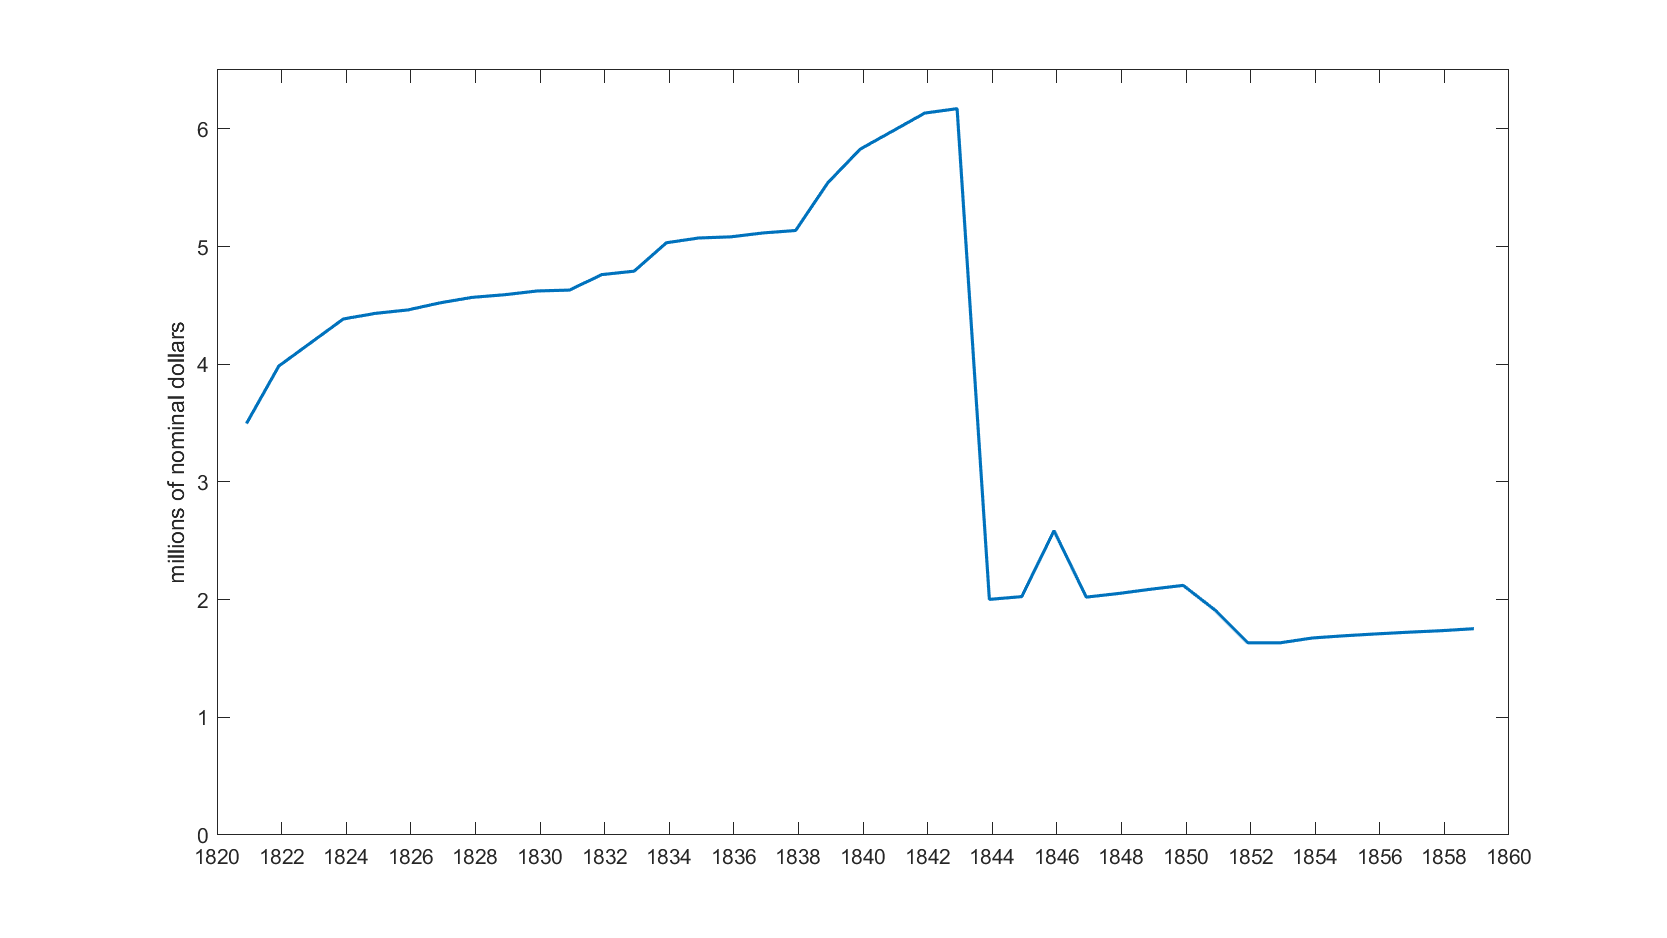
\includegraphics[scale=0.50]{penn_stocks.png}}
\caption{Pennsylvania State Assets, Not Including Public Works}
\label{fig:penn_assets}
\end{figure}

\clearpage

\section{Losses on the Canals and Railroads}

\begin{itemize}
 
 \item In response to the success of the Erie Canal, in February 1826, the Pennsylvania Legislature authorized the Main 
 Line of Public Works to begin the building of canals from Philadelphia to Pittsburgh.
 
\item Between 1830 and 1857, the State of Pennsylvania operated and 
collected toll revenue on nine divisions of the Pennsylvania Canal and two railroads. 
\begin{center}
\begin{tabular}{lrr}
    & Length (in miles) & Cost of Construction \\
\cline{2-3}
{\sc Railways} \\
\hspace{3mm} Columbia and Philadelphia        &  82    &  \$5,277,278\STRUT\\
\hspace{3mm} Allegheny Portage                &  36    &    2,708,672\\
\cline{2-3}
\hspace{6mm}{\em Railway Total}         &  118   &  \$7,985,950\\                                

{\sc Pennsylvania Canal}\STRUT \\
\hspace{3mm} Eastern Division            &  45    &  \$1,737,285\STRUT\\ 
\hspace{3mm} Juniata Division            & 128    &    3,575,966\\
\hspace{3mm} Western Division            & 103    &    3,173,432\\
\hspace{3mm} Delaware Division           &  60    &    1,454,937\\ 
\hspace{3mm} Susquehanna Division        &  41    &      897,161\\
\hspace{3mm} North Branch Division       &  73    &    1,598,379\\
\hspace{3mm} West Branch Division        &  76    &    1,832,583\\
\hspace{3mm} French Creek Division       &  49    &      817,780\\
\hspace{3mm} Beaver Division             & 30     &      519,365\\
\cline{2-3}
\hspace{6mm}{\em Canal Total}     &  605   &  \$15,606,888\\                                

Unfinished Improvements           &      &  \$8,695,044\STRUT\\
Other Costs                       &      &      254,384\\
\cline{2-3}
\hspace{6mm}{\em Grand Total}     &     &  \$32,542,268\\                                
\end{tabular}
\flushleft{\footnotesize Source: \cite{penn_pub_works_cost_1854}.}
\end{center}

\item The average cost to build the Pennsylvania Canal was \$25,797 per mile.

\item For comparison, the Erie Canal was 363 miles and cost \$7,143,000 (or \$19,678 per mile) to construct.

\item In 1854, the State Treasurer and Auditor General 
detailed the expenditures on and revenues  
from these canals and railroads as well as the unfinished projects through 1853.  
\begin{itemize}

\item For each of the 11 canals and railroad, they report annual 
disbursements ``attendant consequent upon the operation of the works." These 
are ``variable costs'' for operating these canals and railroads and line up 
with numbers recorded in the annual reports of the State Treasurer, the Auditor 
General and the Canal Commission.  These expenses include maintenance and wages 
paid to toll collectors, weigh-masters, and lock-keepers.

This series of variable costs is reported in the red line (labeled Running 
Expenditures) in figure~\ref{fig:penn_canal_rev_exp}.

\item They also report the annual revenue.  This series lines up with the 
toll revenue reported elsewhere. I add canal fines to the toll revenue, 
and plot this series as the blue line in 
figure~\ref{fig:penn_canal_rev_exp}.  

\item The Treasurer and Auditor estimate that the total interest paid on 
interest for money borrowed to build and run these public works up to 1853 
was \$35.2 million.  They don't provide an explanation of exactly how they 
compute these numbers.  As we can see in figure~\ref{fig:penn_debt}, nearly
all the Pennsylvania State debt was 
incurred to fund internal improvements.  

If we sum the coupon payments made on all the loans issued to pay for internal improvement 
or to pay principal or coupons on past loans from 1820 to 1853, we get 
\$35.2 as well.  Adding our estimate of these interest payments 
to the variable costs series produces the yellow line in 
figure~\ref{fig:penn_canal_rev_exp}.

\item They also report the aggregate cost for building each of these canals 
and railroads.  Summing these costs across the 11 public works comes to 
\$32.5 million.  If we sum all the spending on internal improvements reported 
elsewhere and net out the running expenditures, we get almost \$30 
million.\footnote{I don't know where other \$2 million comes from.}
If we add our series of ``All 
Other Spending" on internal improvements to the yellow line, we get the purple 
line in figure~\ref{fig:penn_canal_rev_exp}.

\item These numbers are summarized in table~\ref{table:penn_canal_rev_exp}.

\end{itemize}

\item Even with our underestimate of the fixed costs of construction, it 
is clear that the losses on the Pennsylvania canals and railroads were large. 
The State spent either \$87 million (their estimate) or \$84 million (our 
estimate) to build, finance, and run these public works between 1820 and 1853. 
They collected only \$25 million in revenue during this period.

\item In figure \ref{fig:penn_canal_rev_exp}, toll revenue (blue line) and 
running expenses (red line) track each other.  After 1842, toll revenue 
consistently exceeded running expenses.  Nevertheless, toll revenue comes 
nowhere close to covering the interest payments due -- much less recouping 
the costs of construction.

\item From 1842 to 1850, expenditures on internal improvements above those 
for running the canals and railroads were essentially zero.

\item In 1844, the State offered a set of canals and railroads for 
sale at \$20 million.  There were no takers.

\item Again, in 1854, the State put the railways and canals up for sale without success.

\item Then, on June 25, 1857, the State sold the
\begin{itemize}
\item Columbia and Philadelphia Railway  
\item Allegheny Portage Railway          
\item Eastern Division of Canal  
\item Western Division of Canal 
\item some other canals as well -- still need to figure out the details
\end{itemize}
to the Pennsylvania Railroad Company for \$7.5 million.

\item The following year, the remainder of the canals and railroads were sold to the
Sunbury and Erie Railroad Company for \$3.5 million. I don't see either of 
these payments in the accounts.  Perhaps these payments show up in the 1860s. 

\end{itemize}

\begin{figure}
\center{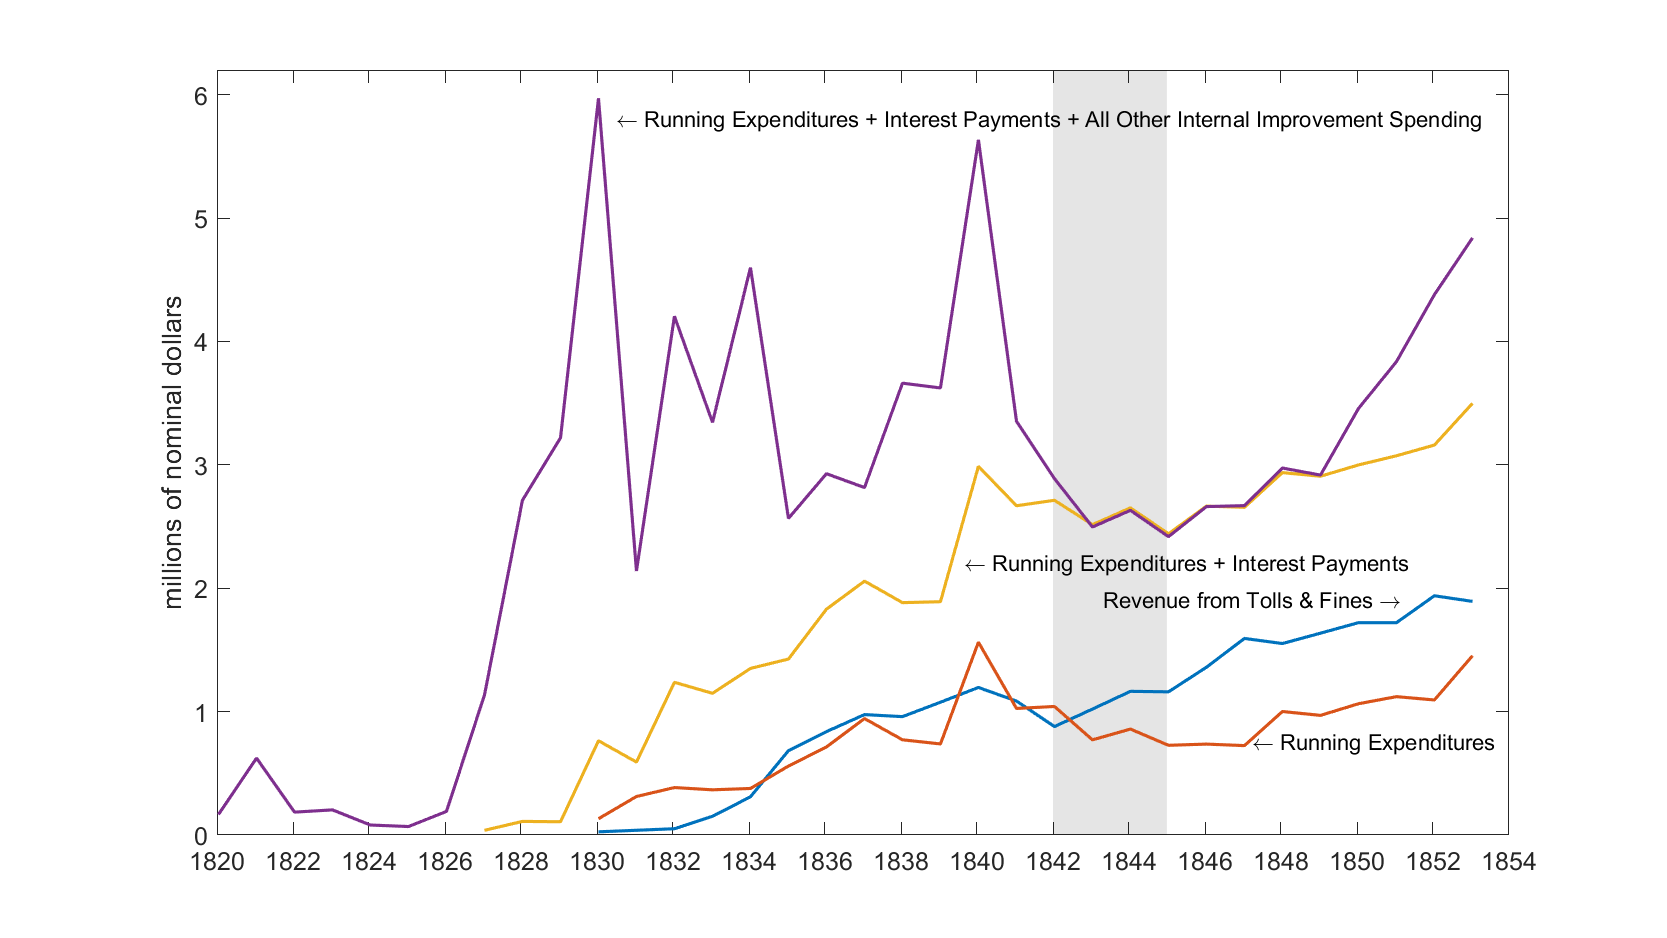
\includegraphics[scale=0.50]{penn_canal_revenue_expend.png}}
\caption{Canal and Railroad Revenue and Expenditures}
\flushleft{\footnotesize The period of the default, 1842-1844, is shaded in grey.} 
\label{fig:penn_canal_rev_exp}
\end{figure}

\begin{table}
\begin{center}
\begin{tabular}{lrr}
&  Official Numbers   & Our Numbers\\
\hline
Expenses Incurred to Run \STRUT\\
the Canals and Railroads: 1830-1853 &    \$19,447,654   &  \$19,477,654\\
Interest Payments on Canal \STRUT \\
and Railroad Debt: 1827-1853      &      35,157,796   &    35,231,591\\
Cost to Build the Canals \STRUT \\
and Railroads: 1820-1853            &      32,542,268   &     28,954,372\\
\hline
Total Costs                                                  &  \$87,147,717     &   \$83,663,617\STRUT\\
\\
Revenue from Tolls                                           &  \$24,995,632     &    \$24,995,632  
\end{tabular}
\caption{Aggregated Fixed Costs, Variable Cost and Revenue for the Pennsylvania Canals and Railroads}
\label{table:penn_canal_rev_exp}
\end{center}
\flushleft{\footnotesize Source: \citet{penn_pub_works_cost_1854}.}
\end{table}

\section{The 1841-1844 Crisis}

\begin{figure}
\center{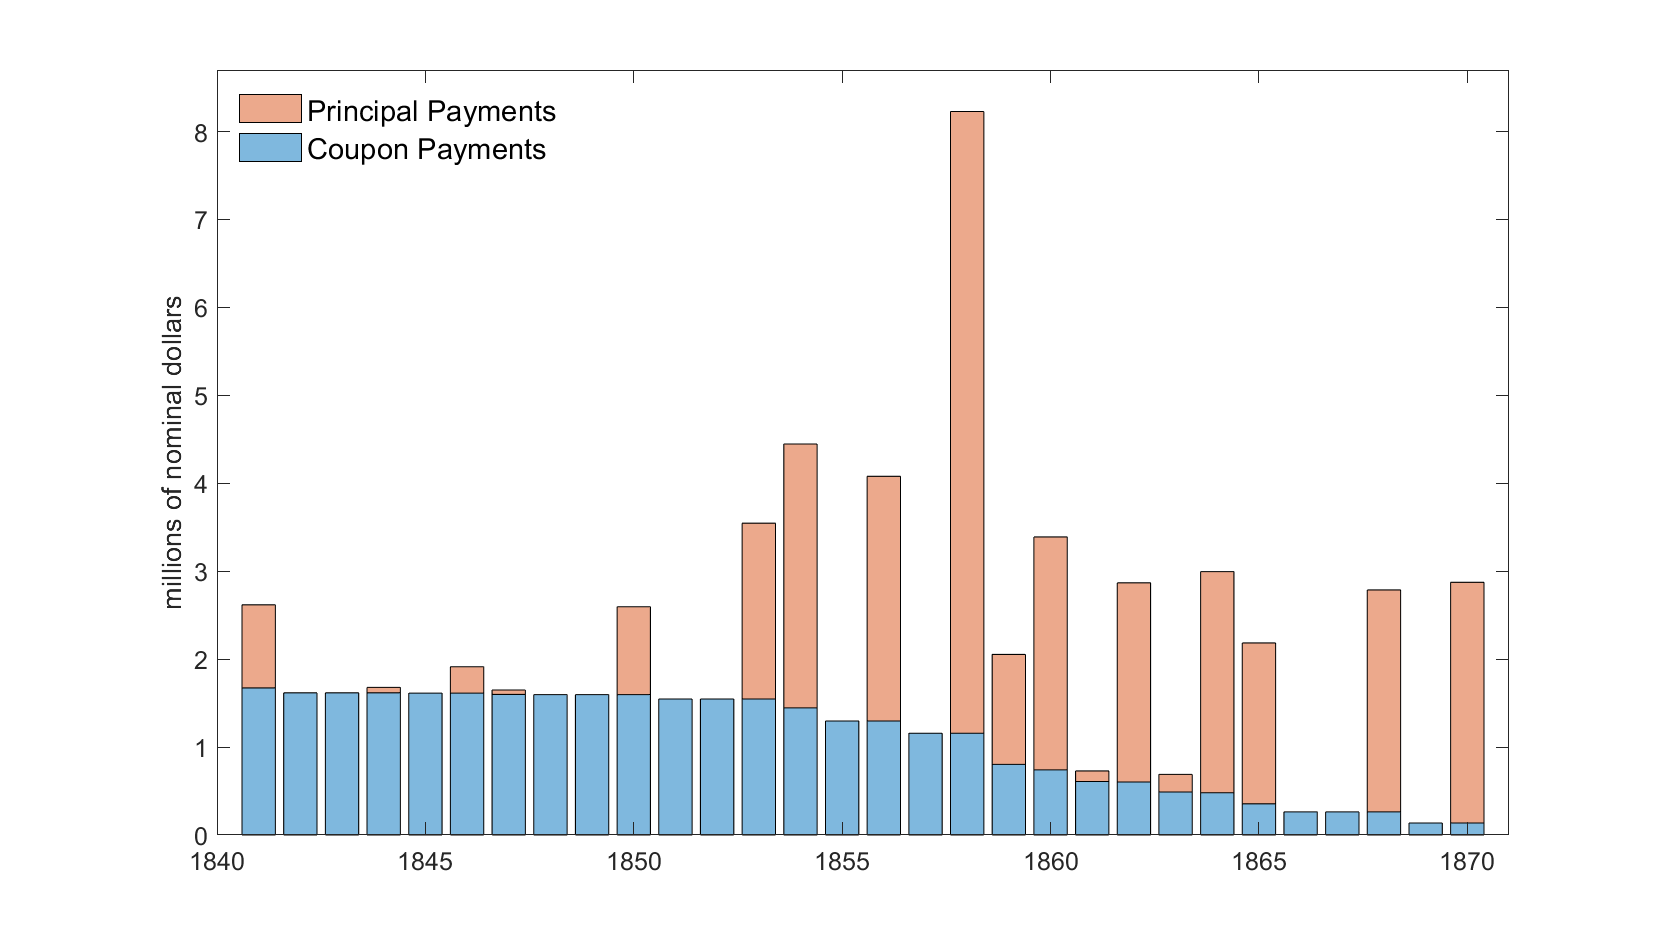
\includegraphics[scale=0.50]{penn_debt_service_profile_1840.png}}
\caption{Debt Service Profile for December 1840}
\label{fig:dsp_1840}
\end{figure}

In figure~\ref{fig:dsp_1840} I plot the debt service profile 
for the debt as of December 1840.  Pennsylvania did not have a lot 
or principal payments due in 1840s.  It was the promised coupon 
payments that killed'em. 


\subsection{1841: Relief Notes}

\begin{itemize}

\item In 1838, 1839, and 1840, the State ran budget deficits of \$2.9, \$2.9, and \$4.8 million.

\item In 1841, the budget deficit was \$2.5 million.  Expenditures included  
\begin{itemize}
\item loan repayments \$675,000
\item interest \$1,707,000
\item internal improvements \$1,710,000
\item other expenditures \$803,000
\end{itemize}
for a total of \$4.2 million.

That year, the State brought in only \$1.7 million in revenue.

\item They were unable to borrow from the bond market.  I need to get the story.

\item In 1841, Pennsylvania did not default on its promised interest payments or other 
obligations, but to do so, it had to borrow money from banks, which could then, 
in turn, issue small-denomination relief notes.

\begin{itemize}

\item The Pennsylvania Relief Note Act of 1841 (formally the Act of May 4, 
1841), an emergency measure passed by the Pennsylvania General Assembly, 
authorized a \$2.22 million ``relief loan.''  To secure the loan, the state 
authorized chartered banks to issue small-denomination paper currency known 
as ``relief notes''. These notes were issued in denominations of \$1, \$2, 
and \$5, which were generally illegal under existing laws that banned 
small-denomination bank notes.

\item Banks that subscribed to the loan were permitted to issue these notes 
up to the amount of their subscription. In exchange, they were granted relief 
from certain state taxes and penalties for suspending specie payments. 

\item The notes were made receivable for all debts due to the Commonwealth, 
effectively making them a state-backed currency.

\item The outstanding quantity of these notes is plotted in purple in figure~\ref{fig:penn_debt}.

\end{itemize}
\end{itemize}

\subsection{1842-1844: Interest Certificates, Domestic Creditors, and Asset Sales}

\begin{itemize}

\item The interest due in February 1842 was paid, but by August 1, 
the treasury was exhausted.

\item \cite{English_1996} dates the default as August 1842.  That lines up.  
He dates the resumption as February 1845.
 
\item The Commonwealth was unable to borrow the \$870,000 authorized by the 
Act of July 27, 1842. Need to explain the inability to borrow.  
Clearly they were shut out of the bond market in 1841.

\item The State Treasurer issued to bondholders certificates of stock equal 
to the amount of interest then due. These certificates bore interest at five 
percent and were payable on August 1, 1843.  See the green region in 
figure~\ref{fig:penn_debt}.

\item The act also provided for the partial payment of claims held by 
contractors and others employed on the public works. These claimants were 
classified as \emph{domestic creditors}.  See the light blue region in 
figure~\ref{fig:penn_debt}.

\item County commissioners were instructed, upon collecting county rates and 
levies, to impose an additional tax of one mill on the dollar on both real 
and personal property for the use of the Commonwealth. This provision was 
intended to remain in force for one year only.

\item The governor was further directed to solicit proposals for the sale of 
the public works and to submit such proposals to the legislature. These 
efforts failed to generate any buyers.

\item At the next interest date, February 1, 1843, the treasury again lacked 
sufficient resources to meet its obligations, and provision was once more 
made for the issuance of stock in payment of interest.

\item In April 1843, a commission was appointed with authority to sell any or all 
state stock held by the Commonwealth in incorporated companies. All of the 
state’s bank stock and other holdings were subsequently sold, 
The face value of these stocks was \$4,169,440.45. 
The State received \$1,395,411.84 (1/3 of the face value) in this sale.  
See figure~\ref{fig:penn_assets}.

\item During the same year, the Commonwealth also received \$60,313.27 
from the federal government as its share of proceeds from the sale of public 
lands.

\item I don't understand the resumption of payments.  Relief notes,  Interest certificates, and unpaid domestic creditors
and a few (\$800) domestic creditors are still outstanding in 1860.  Were some creditors given priority over others?


\end{itemize}

\section{Ownership of Pennsylvania State Debt}

\begin{itemize}

\item Promises needed to be broken.  The State could:  
\begin{itemize}
\item fail to pay domestic creditors,
\item fail to pay foreign bondholders, or
\item raise taxes on its citizens 
\end{itemize}

\item This led to a discrimination problem that was an echo of the one Hamilton faced in 1790:
\begin{itemize}
\item Failing to pay domestic creditors or raising taxes risked immediate electoral backlash and more social unrest.

\item Failing to pay foreign bondholders carried reputational costs, but those costs were diffuse and delayed.
\end{itemize}

\item I don't have the full story of this discrimination was resolved.  There was no formal restructuring of the debt as far as I can tell.  

\item In 1842, there was \$34,454,356.47 in Pennsylvania debt outstanding.

\end{itemize}

\begin{center}
\begin{tabular}{lr}
Pennsylvania     &  \$9,635,613.47\\
Other US citizens &  1,080537.60\\
Foreigners        &  23,738,206.00\\
\hline
Total             &  \$34,454,356.47
\end{tabular}
\end{center}
\flushleft{\footnotesize Source: \cite{holders_state_debt_1842}.}


The top five other states were
\begin{center}
\begin{tabular}{lr}
New York    &  \$417,856\\
Massachusetts &  129,000\\
District of Columbia  & 86,220\\
Virginia              & 84,700 \\
Delaware              & 76,180
\end{tabular}
\end{center}
\flushleft{\footnotesize Source: \cite{holders_state_debt_1842}.}

The top five foreign countries were
\begin{center}
\begin{tabular}{lr}
England           &  \$20,026,458\\
Holland           &  1,822,266\\
France            &  570,000\\
West Indies       &  563,161\\
Switzerland       &  239,677\\
\hline
\end{tabular}
\end{center}
\flushleft{\footnotesize Source: \cite{holders_state_debt_1842}.}


\section{Bond Prices}

\begin{figure}
\center{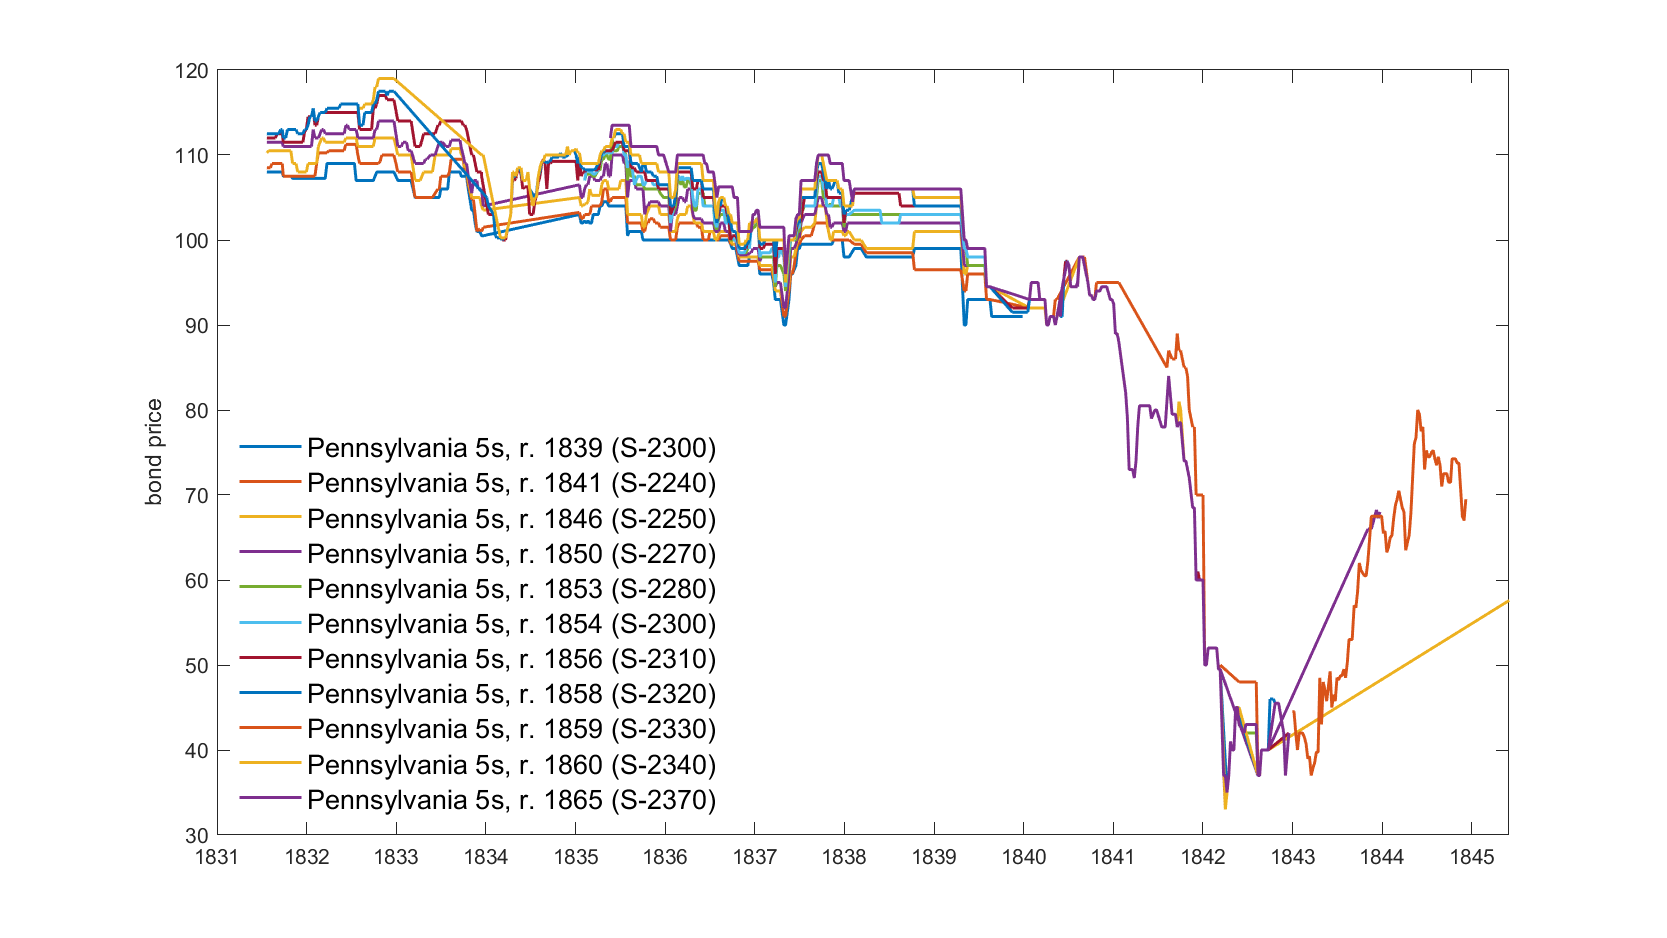
\includegraphics[scale=0.50]{penn_state_debt_prices.png}}
\caption{Prices of Various Pennsylvania State Bonds}
\flushleft{\footnotesize Source: \cite{Sylla_Wilson_Wright}.}
\label{fig:penn_bond_prices}
\end{figure}

\section{Unit of Account Issues}

\begin{itemize}

\item In May 1837, banks in Pennsylvania and across the United States 
suspended specie payments  in response to the panic and financial 
crisis of that year.

\item In July 1839, the legislature passed a resolution that the State would 
pay interest in ``lawful money'' (which I think in this case meant specie) 
and if the Treasury paid interest in any currency of less value than legal 
money, it must make up the difference.  We see evidence of this "making up 
the difference" in the Treasury records.

\item There is probably more to this story.  \cite{worthington_1887} has a 
discussion of this on page 47.

\end{itemize}

\newpage

\section{Data Sources}

\begin{itemize}

\item The data for revenues, expenditures, state balances, and debts are 
from various issues of the {\em Report on the Finances of the Commonwealth of 
Pennsylvania for the Year 18XX Made to the Legislature by the Auditor General}.

\item For some years, the same data are also reported in the {\em Report of the State Treasurer upon the Finances of Pennsylvania}.

\item Unlike other state fiscal datasets, our records are consistent with the budget constraints presented at the start of this memo.

\end{itemize}


\clearpage
\bibliography{war_finance}

\end{document}

